\subsubsection{Embedded Runge-Kutta}

\begin{table}[!ht]
  \centering
  \caption{Oscillation test: errors analysis of explicit embedded Runge-Kutta solvers}\label{tab:oscillation_errors_emd_rk}
  \begin{subtable}[b]{0.40\textwidth}
    \centering
    \caption{7 stages}\label{tab:oscillation-emd-rk-7}
    \resizebox{1.00\textwidth}{!}{%
    \begin{tabular}{ccccc}
      \toprule
      {\sc Mean Time Step} & {\sc Error X} & {\sc Error Y} & {\sc Order X} & {\sc Order Y} \\
      \hline
      7352.9               &  0.626E-01    &  0.622E-01    & /             & /             \\
      3759.4               &  0.482E-02    &  0.480E-02    & 3.82          & 3.82          \\
      2272.7               &  0.793E-03    &  0.786E-03    & 3.59          & 3.59          \\
      1379.3               &  0.393E-04    &  0.390E-04    & 6.02          & 6.02          \\
       618.8               &  0.216E-05    &  0.213E-05    & 3.62          & 3.62          \\
       356.0               &  0.252E-06    &  0.249E-06    & 3.89          & 3.88          \\
      \bottomrule
    \end{tabular}}
  \end{subtable}\\
\end{table}

\begin{figure}[!ht]
  \centering
  \begin{subfigure}[b]{0.45\textwidth}
    \centering
    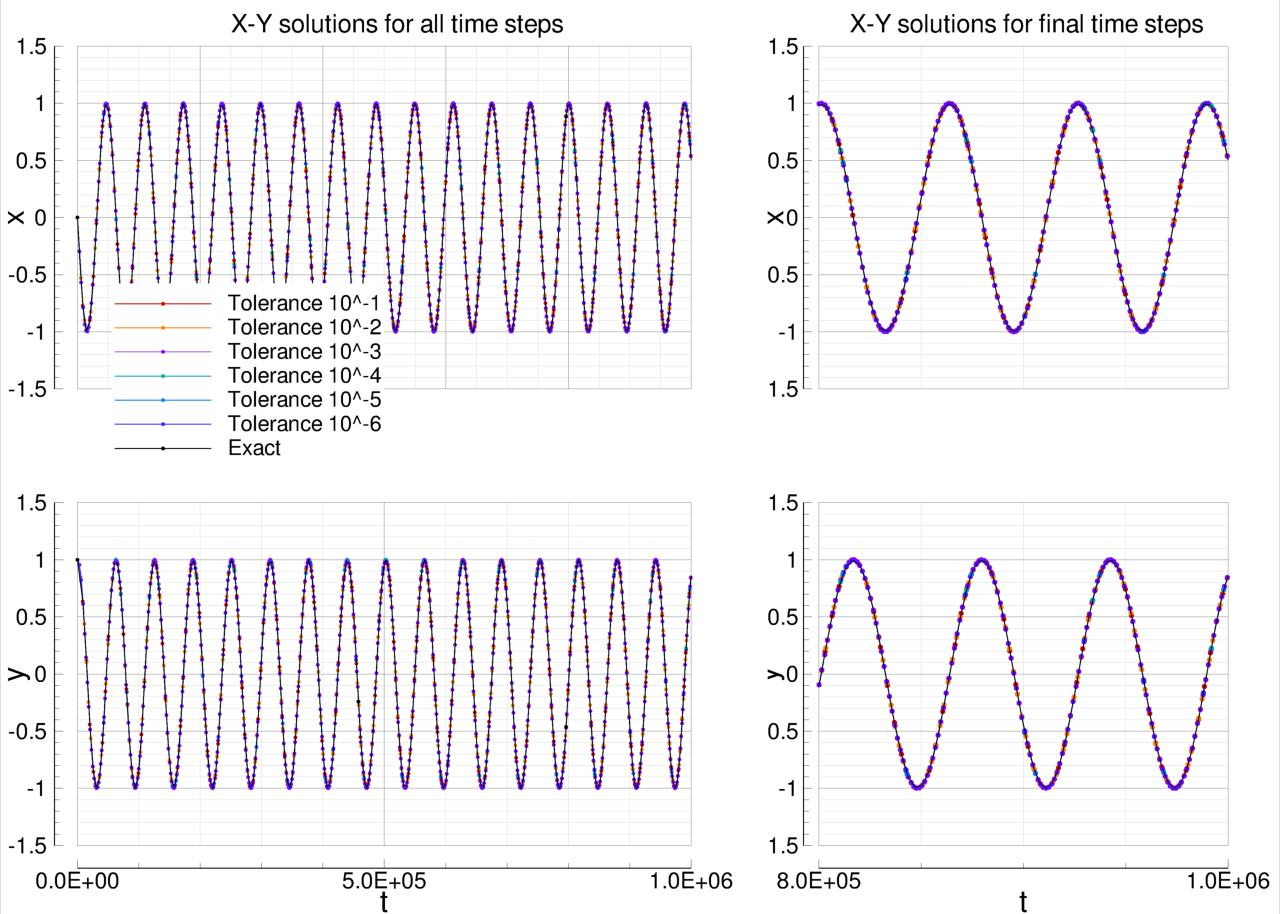
\includegraphics[width=1.00\textwidth]{errors-analysis/oscillation/errors_analysis-oscillation-emd-runge-kutta-7.png}
    \caption{7 stages}\label{fig:results-oscillation-emd-runge-kutta-7}
  \end{subfigure}\quad%
  \caption{Oscillation equations solutions computed by means of embedded Runge-Kutta solvers}\label{fig:results-oscillation-emd-runge-kutta-1-7}
\end{figure}
